\documentclass[12pt]{article}
\usepackage{pslatex} % Font Times New Roman

\usepackage{amsmath,amssymb,amsfonts,amsthm,fancyhdr,lastpage}
\usepackage{makeidx, graphicx}

\setlength{\textheight}{9.0in}
\setlength{\topmargin}{-.5in}
\setlength{\textwidth}{6.5in}
\setlength{\oddsidemargin}{-.0in}
\setlength{\parskip}{6pt}


\renewcommand{\headrulewidth}{0pt}
\setlength{\headsep}{.35in}
\addtolength{\headheight}{2.5pt} 

\usepackage{graphicx}

\begin{document}

\title{Representing Kekule Cells in Stable Molecules}
\author{Aaron Germuth and Alex Aravind \\\\  
Department of Computer Science \\
University of Northern British Columbia \\
E-mail: (germuth,csalex)@unbc.ca}
\maketitle


\begin{abstract}

Silicon transistors may slowly be reaching their minimum size. Possible alternatives to allow the continual decrease of circuitry size are desired. One possibility is the use of $\pi$ conjugated hydrocarbons as circuitry elements.  Certain polycyclic polyunsaturated hydrocarbons have already shown promise in this area. Alternating paths of double and single bonds in $\pi$ conjugated hydrocarbons have to shown the ability to conduct electricity. An alternating path can be toggled by sending a soliton across it. When such a path is toggled, other alternating paths can be created or destroyed. This suggests a possible switching behavior. Kekul\'e theory attempts to characterize this phenomenon. The Kekul\'e cell captures the switching behavior in a mathematical way. All possible cells have been reduced to a classification. Therefore, if we can find a molecule for every classification, we have found a molecule for every possible switching behavior. We attempt to, given any cell, find a suitable molecule which has that cell. A genetic algorithm is used to evolve a population of graphs towards the required switching behavior. Most graphs obtained from the genetic algorithm resemble realistic graphs which in theory, could be used as circuitry elements. The genetic algorithm is capable of quickly producing results for all cells of rank 5 or lower, and most cells of rank 6.

\end{abstract}

\section{Introduction}

First a review of organic chemistry is given in section 1.1. A brief review of graph theory is given in Section 1.2. Section 1.3 outlines the current need for smaller computational elements. Section 1.4 begins to introduce molecular electronics. Section 1.5 introduces Kekule Theory.  Definitions for many terms are given after each subsection.

\subsection{The Chemistry}

Carbon is the $6^{th}$ element of the periodic table and backbone of all organic molecules. It is tetravalent, meaning it has 4 valence electrons available to form chemical covalent bonds. In such bonds, atoms share electrons relatively equally between them. For example, a neutral chlorine atom has 7 electrons in its outer shell. According to the octet rule, most atoms are stable with 8 electrons. For example, chlorine commonly dimerizes with itself, sharing one electron each way to give each chlorine 8 shared electrons in its outer shell (see Figure \ref{fig:chlorine}).

\begin{figure}[ht!]
\centering
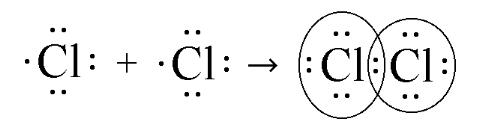
\includegraphics[width=110mm]{chlorine.jpg}
\caption{This shows the forming of a covalent bond between two neutral chlorine atoms. Each atom initially has 7 electrons, until they each share an electron with each other, yielding them both 8 electrons. Carbon only possesses 4 electrons in it's neutral state, and therefore usually shares electrons with 4 other atoms.}
\label{fig:chlorine}
\end{figure}

Each possible bonding partner will contribute a single electron to the covalent bond, meaning carbon, who has only 4 electrons, will have 8 electrons in its full valency. This is considered a full octet, and the stable configuration of carbon. However, 4 bonding partners is not always needed in order to be stable. If Carbon was bonded to 3 other atoms, but one of them was able to share 2 electrons (a double bond), carbon would still have a full valency of 8 electrons (see Figure \ref{fig:C02}).

\begin{figure}[ht!]
\centering

\includegraphics[width=60mm]{c02.jpg}
\caption{This figure shows the Lewis Structure of Carbon dioxide. Each oxygen is capable of sharing 2 electrons. Since carbon has 4 electrons normally, they are split evenly between the oxygen atoms. This results with every atom having 8 electrons. Carbon is said to be double-bonded to each oxygen.}
\label{fig:C02}
\end{figure}

\subsection{The Electron}
Electrons can't be clearly identified as either a particle, or a wave. In fact they show traits of both entities. Electrons have mass, indicating they are indeed a particle. However, physical experiments such as the two-slit experiment have shown that electrons can form an interference pattern, an attribute only seen by waves, such as light. This phenomenon is called the wave particle duality. 

Werner Heisenberg then postulated an uncertainty principle, saying you may only know either an electrons position, or momentum at one point in time. In this way, you can only ever know half the information about where and how an electron is traveling. However, electrons are known to orbit the atom. Because of this, electrons are said to be in 'orbitals' around the atom. These are regions of 3D space where the electron is most likely to appear, most of the time. These electron probability clouds are only a guess as to where the electrons should be, when orbiting an atom.
 
\subsection{Electron Orbitals}
According to the Valence Bond Theory, single and double bonds have different electron structures. Single bonds are named "sigma ($\sigma$) bonds", and are caused by the head-on overlapping between atomic orbitals. Sigma Bonds are the strongest type of covalent bond. Double bonds are named "pi ($\pi$) bonds", and result from electron overlap in the nodal plane of both atoms. Double bonds are weaker, but still resilient. See Figure \ref{fig:bonds}.

\begin{figure}[ht!]
\centering
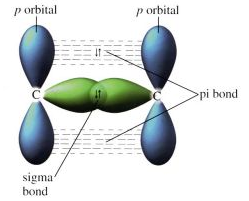
\includegraphics[width=75mm]{bonds.png}
\caption{The green electron overlap constitutes a sigma bond. Where as each set of dotted lines betewen the blue electron cloud constitutes a pi bond.}
\label{fig:bonds}
\end{figure}

Many organic molecules display alternating paths of single and double bonds. In this configuration, every atom is connected with precisely one double bond. This is named conjugation, and can increase molecular stability. In these types of bonds, electrons of the $\pi$ orbitals are free to traverse the entire conjugated section. 

Conjugation usually implies the possibility of different resonance structures, where every double bond shifts in one direction to obtain a different representation of the same molecule. The amount of such resonance structures is a measure of stability.  The 'real' moleculac structure is a weighted average of all resonance structures, with the most stable resonance structures as the most important contributors.

Each of the nodal lobes involved in pi bond conjugation allow their electrons to delocalize across the conjugation. Since electrical current is the flow of electrons, such alternating paths are postulated to be electrically conductive \cite{H13,HK88}. When certain electricity (specifically a `soliton', explained later) is ran through a conjugated system, all single and double bonds are interchanged \cite{HK88}. 

\subsection{Chemistry Definitions}

\begin{description}
\item[Organic Compound] An organic compound is any member of a large class of gaseous, liquid, or solid chemical compounds whose molecules contain carbon.
\item[Electron] A subatomic particle with a negative elementary electric charge. 
\item[Valence Electron] An electron that can participate in the formation of a chemical bond; 
\item[Tetravalence] The state of an atom with four electrons available for covalent chemical bonding.
\item[Covalent Bond] A chemical bond that involves the sharing of electron pairs between atoms.
\item[Octet rule] A chemical rule of thumb that states that atoms tend to combine in such a way that they each have eight electrons in their valence shells.
\item[Dimerize] The process of two structurally similar chemical compounds binding together.
\item[Lewis Structure] Diagrams that show the bonding between atoms of a molecule by drawing each electron as a 'dot'.
\item[Double bond] A chemical bond between two chemical elements involving four bonding electrons instead of the usual two.
\item[Wave] A disturbance or oscillation which travels through space and matter. Accompanied by a transfer of energy.
\item[Two Slit Experiment] A experiment demonstrating that matter (such as electrons) can exhibit characteristics of both waves and particles.
\item[Uncertainty Principle] A mathematical inequality stating a fundamental limit to the precision of which you can know information about subatomic particles. If the position is know, the momentum cannot be, and vice versa.
\item[Atomic Orbital] A mathematical function which describes the wave-like behavior of electrons orbiting an atom's nucleus. May refer to the physical region of space the electron may occupy.
\item[Valence Bond Theory] A basic theory developed to use to explain chemical bonding. It explains how the atomic orbitals of the atoms combine to give individual chemical bonds when a molecule is formed. 
\item[Sigma Bond] The strongest type of covalent chemical bond. They are formed by head-on overlapping between atomic orbitals. Commonly referred to as a 'single bond'.
\item[Pi Bond] Commonly referred to as a 'double bond'.
\item[Conjugated System] A system of connected p-orbitals with delocalized electrons in compounds with alternating single and multiple bonds
\end{description}

\subsection{Graph Theory}

Graph Theory, a discipline of mathematics and computer science, is the study of graphs. Graphs in this context model relations between objects. Such objects are represented using nodes. Relations between them are called edges. Relations between objects can be single or bidirectional (see Figure \ref{fig:graph}).  

\begin{figure}[ht!]
\centering
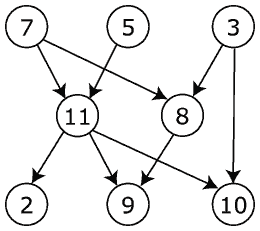
\includegraphics[width=75mm]{graph.png}
\caption{This graph is composed of 8 nodes. Nodes are sometimes labeled, in this case with numbers. Edges in this graph are directed (they can only be traversed in one direction), and so this graph is called a directed graph.}
\label{fig:graph}
\end{figure}

Typically graphs are drawn using circles for each node, and lines for each edge. If an edge goes from one node to itself, it is called a loop. Multiple edges can occur when there is more than one edge to travel from one node to another. 

A simple graph has no loops or multiple edges. Graphs with only bidirectional edges are called undirected graphs. Graphs whose edges have a single direction are called directed graphs. A path is a sequence of adjacent nodes and edges through a graph. A cycle is a path whose starting point is also it's ending point. Two nodes are connected if there is a path between them. A graph is connected if all node pairs are connected. A subgraph is a graph whose vertex and edge set are a subset of the original graph. 

A matching is a subgraph consisting of a set of pairwise non-adjacent edges. This means no two edges share a common vertex. A perfect matching is a matching which matches all verticies of the graph. Every node of the graph is incident to exactly one edge of the matching. Efficient algorithms exists to compute a perfect matching.

\subsubsection{Graph Definitions}

\begin{description}
\item[Graph] A tool to model relations between objects. Consists of nodes and vertices.
\item[Loop] An edge whose starting and ending point are the same node.
\item[Multiple Edges] When there are more than one edge between two adjacent nodes.
\item[Simple Graph] A graph without loops or multiple edges. 
\item[Undirected Graph] A graph where all edges are bidirection.
\item[Directed Graph] A graph where all edges have single direction.
\item[Path] A sequence of adjacent nodes and edges through a graph.
\item[Cycle] A path whose endpoint and starting point are the same vertex. Cycle must contain atleast 2 nodes.
\item[Connected Graph] A graph where all pairs of nodes contain a to one another.
\item[Subgraph] A graph containing a subset of nodes and edges from another graph.
\item[Perfect Matching] A matching where all nodes of the graph are matched.
\end{description}

\subsection{Silicon Electronics}

%this whole paragraph semi plagarizes
As the use of electronic systems become more vital to our society, demands for new technological developments are ever increasing. %First sentence needs to be reworded in our own words. 
A large portion of the current technological development has been spent reducing the size of the conventional silicon transistor. Smaller transistors allow faster computation. Approximately every 2 years, twice the amount of transistors have been able to fit in the same space.

Gordon Moore, predicted this trend (see Figure ~\ref{fig:MooresLaw}) in 1965 \cite{Moore}, and since then it has been accurate. However, there are signs which show this exponential progress is coming to an end \cite{MooreEnd}. Conventional silicon transistors may soon reach their minimum physical size. As they get smaller, so does the amount of current which runs through them. The amount of leakage current (current lost through transit) is approaching the order of magnitude of the actual current running through the transistor itself \cite{v06}. At this point, current silicon transistors will no longer be able to continue decreasing in size.

\begin{figure}[ht!]
\centering
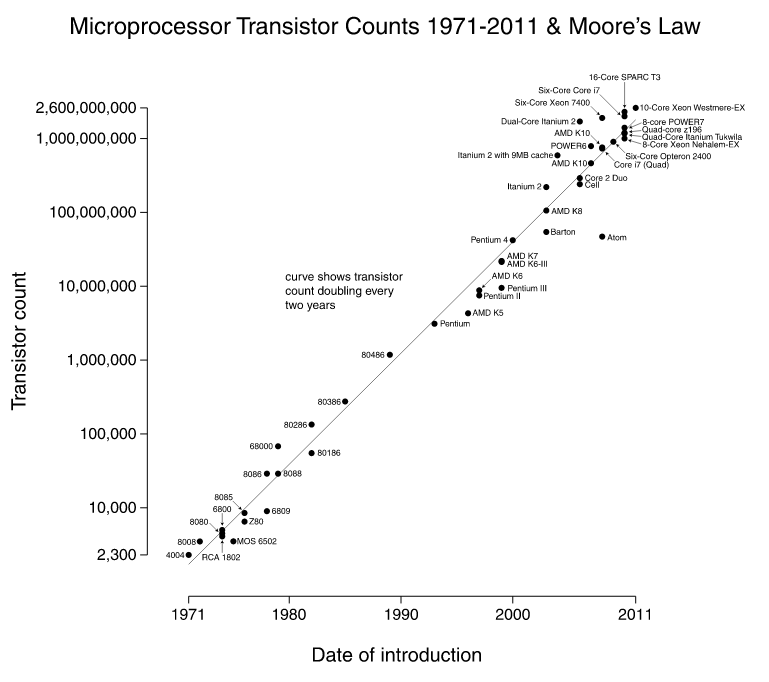
\includegraphics[width=110mm]{MooresLaw.png}
\caption{Plot of CPU transistor counts against dates of introduction, on a logarithmic vertical scale.}
\label{fig:MooresLaw}
\end{figure}

Unless a new innovation which allows scientists to overcome the current fundamental physical limitations of silicon transistors, a new approach is needed. 

\subsubsection{Definitions}

\begin{description}
\item[Transistor] A semiconductor device used to amplify and switch electronic signals or electrical power. The fundamental building block of modern electronics.
\item[Capacitor] A passive electrical component used to store energy in the form of electrostatic fields.
\item[Leakage Current] The gradual loss of current from charged capacitors. 
\end{description}

\subsection{Molecular Electronics}

One alternative possibility to allow smaller circuitry is to use single molecules as computational elements. $\pi$ conjugated systems have been suggested as delocalization allows electrons to move freely over a conjugated area. Molecules must also display charge transmission, the ability to carry electrical charges. One technique to allow charge transmission in molecules is doping. 

%more re-wording needed here
Doping involves introducing an impurity into an electrical conductor to modify its electrical properties. Often such an impurity can increase the conductance. Conductive polymers can be doped by adding chemical reactants to oxidize, or sometimes reduce, the system so that electrons are pushed into the conducting orbitals within the already potentially conducting system. This can allow charge transmission through a molecule. 

%more re-wording here
A special kind of charge transmission is the use of solitons. A soliton is defined as a self-reinforcing solitary wave, maintaining its shape while traveling at a constant speed. In this case, the wave could be considered a pair of electrons, 'hopping' across all double bonds. As a soliton migrates, it displaces electrons from nearby double bonds to single bonds, effectively inverting the conjugated system (all double bonds become single, and vice versa).

Much effort has gone into molecular circuitry. It is viewed as the ultimate reduction in circuitry size. The earliest progress was spent trying to make molecular equivalents of the current silicon approach (wires, transistors, switches, and logic gates). 

An electrical wire is a passive element, intended to interconnect separate components. Large polymers such as phenyl-enthylnylanthracene has been suggested as wires, both theoretically and experimentally. Usually such wires are tested using gold electrodes with resilient thiol-Au bonds. 

A rectifier (or diode) is an electric device which converts an alternating current (AC) into a direct current (DC). Molecular electronics have used complex conjugated molecules to achieve rectification. Such molecules only conduct electricity after a certain voltage is reached. This filters the output to only show voltage above certain threshold, rectifying the output to an asymmetric flow of current. 

Other silicon based components have been mirrored as well. Other solutions include wires \cite{9}, diodes \cite{10,11}, resistors \cite{12,13}, transistors \cite{14, 15, 16, 17}, and switches \cite{18, 19}. However, considerable research has gone into using molecules as logic gates, rather than constructing logic gates out of multiple transistors or diodes. This began the search for molecular switches. 

Early approaches involed de Silva et al showing a crown-ether molecule which models an AND gate. The molecule fluoresces, only if both sodium and hydrogen ions have bound to it. In this way, the florescent output models an AND gate. All 16 logic operations can now be realized using the field of photophysical, photochemical, and electrochemical processes. 

The main problem with this approach is that most molecules are either based on optical input and/or operating in a solution environment. However, if logic gates are actually to be implemented, they must be able to operate in solid-state electronics (not a solution environment). Ideally, molecules could use current itself as input and output, rather than optics or chemical reactions. 

Many proposals have been made with such features. The change transmission property of certain conjugated molecules can be used as a switching mechanism. Aviram and Ratner composed a rectifying diode, which functioned like a AND gate using current-voltage levels. Joachim et al, showed, in theory, a single molecule which can act as an OR or a NOR gate, depending on an additional input. Other solutions include AND\cite{20} , OR\cite{21}, IF THEN (implication)\cite{22}, NAND\cite{23}, and NOR\cite{24}. Despite promising results, Ellenbogen and Love showed that large and somewhat unrealistic molecules would be required for the design of standard logic gates from related wires and diodes. 

\subsubsection{Definitions} 

\begin{description}
\item[Charge Transmission] The ability to transmit electrical charges.
\item[Doping] Adding an impurity to a conductor to change its electrical properties, often increasing electrical conductance.
\item[Polymer] A large molecule composed of many repeating subunits, known as monomers.
\item[Conductive Polymers] Organic polymers which conduct electricity.
\item[Soliton] A self-reinforcing solitary wave which maintains it's shape and speed while traveling.
\item[Diode] An electrical device which filters an electrical current. For example, converting an alternating current into a direct current.
\item[Rectification] The process of filtering an electrical current.
\item[Electrode] An electrical conductor used to make contact with a non-metallic part of a circuit.
\item[Photophysical] The study of physical reactions which either absorb or flouresce light. 
\item[Photechemical] The study of chemical recations which either absorb or flouresce light.
\item[Electrochemistry] A branch of chemistry studying chemical reactions and how electricity may effect them.
\item[Solution] A homogeneous liquid in which chemical reactions take place.
\end{description}

\subsection{Soliton Electronics}

Forrest Carter in 1982 introduced a switching mechanism based on the bond inversion from the traversal of a soliton. A path within a molecule only  facilitates charge transmission when there is an alternating path between the two atoms. When a path within the molecule is inverted from a soliton, other alternating paths may be 'destroyed' or 'created'. This mimics molecular switching.  Groves discussed exactly how soliton switches could be used to constuct logic gates by interconnecting molecules in either series (AND gate) or parallel (OR gate). M. H.  van der Veen \cite{v06} has shown that a single molecule can facilitate all 16 fundamental logic operations. These molecules can even be combined to achieve bi-functional logic with increased complexity.

M. H. van der Veen \cite{v06} describes $\pi$-logic, a way to determine which Boolean operations any $\pi$-conjugated system can preform. All of this allows for, in theory the design of highly compact and complex logic circuits. There still exists many technical problems in applying this potential.

In $\pi$-logic, molecules have terminals which consist of atoms where connections outside the molecule can be attached. $\pi$-conjugated wires \cite{9} or omniconjugated molecules \cite{OmniConj} have been suggested to interconnect separate molecules. A pair of terminals is called a pathway. If there exists an alternating single-double bond path from terminal to terminal, the path is deemed 'open'. Open paths have been shown to conduct electricity to a much higher extent than closed paths \cite{openPath}. A path can be toggled (all single bonds become double bonds and vice versa) by sending an electrical 'soliton' over the path \cite{HK88}. A molecule can contain multiple intersecting paths, and in this way, when one path is toggled, another path may be opened or closed (see Figure ~\ref{fig:acenaptheneHighlighted}).

\begin{figure}[ht!]
\centering
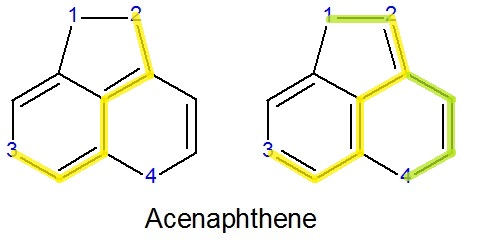
\includegraphics[width=90mm]{AcenaphtheneHighlighted.jpg}
\caption{Acenaphthene displaying switching behavior. There exists an alternating path from terminal 2 to 3 (shown in yellow). When this path is toggled (right diagram), the path from terminal 1 to 4 (shown in green) is also opened.}
\label{fig:acenaptheneHighlighted}
\end{figure}

%(Might exclude this next paragraph) 
To begin the analysis using $\pi$-logic, all possible double bond patterns of the molecule are deduced. Two terminals are selected for an output, and whether the path between them is open or closed represents an output of '1' or '0' respectively. The other terminals are paired, and each pair represents an input of '1' or '0', again depending on the openness of the path. From this you can observe all the different Kekul\'e structures of the molecule and map the inputs to the outputs, resulting with a Boolean function. If the terminals are paired in a different orientation, you may redo the process and have the same molecule represent another Boolean function. 

The main criticism to the soliton approach is its difficulty in actual implementation. Exhibiting any amount of control over electricity at the molecular level is an extreme feat in of itself. Another difficulty is the combination of molecular and conventional electronics. Charge transport through conjugated systems as well as through the macroscopic electrode to the molecule must be fully understood. Proper covalent connections between molecules must also been realized. These interconnections must not change the functionality of the molecule itself. 

\subsection{Kekul\'e Theory}

Kekul\'e theory \cite{H13, HH13} was introduced to investigate and systematize the qualitative switching behavior of certain conjugated systems. In Kekul\'e theory, certain boundary atoms which connect to outside the molecule are called ports.  Alternating pathways through the molecule from one port to another are called channels. A Kekul\'e state is a configuration of bonds such that every node (other than the ports) has precisely one double bond. Ports may or may not have a double bond. Each Kekul\'e state (or resonance structure) of the molecule has a so called port assignment, the set of ports (in that Kekul\'e state) which contain a double bond. A Kekul\'e cell then consists of the set of port assignments for every resonance structure of that molecule (see Figure ~\ref{fig:kekuleCell}). The rank of a cell or molecule is defined as its number of ports.

\begin{figure}[ht!]
\centering
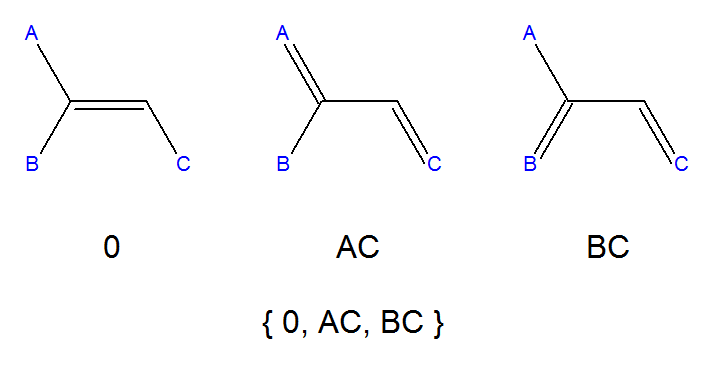
\includegraphics[width=110mm]{KekuleCell.png}
\caption{The Kekul\'e cell of a simple molecule (2-methylbutene). The 3 structures indicate the 3 possible arrangements of double bonds. Each of these could be called either a Kekul\'e state, or a resonance structure. The second row indicates the port assignment (which ports contain a double bond) for each structure, and the third row is the Kekul\'e cell for the entire molecule. This cell has rank 3.}
\label{fig:kekuleCell}
\end{figure}

Molecules are represented by graphs, where nodes resemble atoms and edges resemble bonds. Graphs are simple, undirected, planar graphs. The internal nodes of a graph is all nodes other than the port nodes. A sub-graph is used to show the set of double bonds of any given molecule. To find all possible Kekul\'e states (or resonance structures) of a given molecule/graph, Kekul\'e theory uses perfect matching from graph theory. If every node of the sub-graph has a degree of 1 (indicating they contain precisely one double bond), the sub-graph is said to be perfectly matching, and resemble a resonance structure. Kekul\'e allows near-perfect matchings, as only the internal nodes must contain a double bond, ports are not required. If we find all near-perfect matchings of a graph, we have discovered all Kekul\'e states (resonance structures) of the molecule, along with the port assignment for each one.

Hesselink et al.\cite{HH13} proves that, in any resonance structure, the presence of an alternating path (of single and double bonds) between two ports is completely determined by the Kekul\'e cell. Since alternating paths of single and double bonds conduct electricity, a Kekul\'e cell captures the electrical switching behavior first found by Forrest Carter. Sending a soliton across an open channel in a graph causes the port assignment to change, and therefore the presence of alternating paths.

\subsubsection{Definitions}

\begin{description}
\item[Port] An atom of a molecule which may serve as an input or output of this molecule. It can connect the molecule to other molecules, or molecular wires.
\item[Alternating Path] A sequence of alternating single and double bonds through a molecule.
\item[Kekul\'e State] A resonance structure, with the exception that ports do not have to contain a double bond.
\item[Port Assignment] The set of ports which contain a double bond.
\item[Kekul\'e Cell] The set of port assignment, one for each Kekul\'e state of the molecule.
\end{description}

\subsection{Kekul\'e Cell Classification}

Hesselink \cite{H13} has classified all possible Kekul\'e cells with a given rank. This means any Kekul\'e cell has equivalent switching behavior to a classified one. First, cell invariant operations were defined, modifications that can be done to the cell without changing it's behavior. The renaming of ports was shown to have no effect on the Kekul\'e cell. Cell translation over a port assignment was defined as the symmetric set difference between the port assignment and the cell. The translated cell was also shown to preserve all behavior. 

Hesselink uses these cell invariant operations to converge all possible Kekul\'e cells of a given rank into a single equivalence classification. The first normalization translates all cells to contain the empty port assignment '0'. However, simply containing the empty port assignment is not specific enough, so ports are translated so their 'center' contains the empty port assignment. The 'center' of a Kekul\'e cell is a subset of the cell itself, and consisting of all the 'minimal' h(k).

h(K) is the weight list of each port assignment from a Kekul\'e cell. Ports which are used more often in larger port assignments are given larger weights. Each port's weight is added to obtain the weight of the entire port assignment. The center of a cell becomes the port assignments with minimal weight. 
%not sure about this
These port assignments are the ones translated to contain the empty port assignment. 

The next step of the normalization involves finding all optimal cells. Optimal cells are defined to be centered and have a minimal m(K). To calculate m(K), all ports must have their weight calculated. Then, based on the alphabetical ordering of the ports, a list of their weights is created. This sequence is called a weighted histogram. m(K) is minimal when this list is descending in numerical order. %exact sentence copy
This means ports which occur more often are concentrated near the beginning of the port enumeration. The set of optimal cells is called the raw classification. 

%not sure about this paragraph at all
Finally the raw classification is pruned to yield the final classification. When two or more ports have the same weight, their weighted histogram has many possible permutations which will produce a descending order. Histograms in alphabetical order are chosen over their counterparts to achieve the final classification. 

\subsubsection{Definitions}
\begin{description}
\item[Cell invariant] Operations which have no effect on the switching behavior of the underlying Kekul\'e Cell.
\item[Port Renaming] A cell invariant operation which changes the label of atleast one port. 
\item[Symmetric Set Difference] The set of elements which are in either of the sets but not in their intersection. In Kekul\'e theory, each set is a port assignment, and the members of the set are the ports containing a double bond.
\item[Port Translation] A cell invariant operation. Performed my finding the symmetric set difference between each port assignment of the cell and the translation factor. The translated cell consists of each difference. This new cell has the same switching behavior as the original cell.
\end{description}

\subsection{Searching for Graphs}

The next step is to then, given a Kekul\'e cell, find a corresponding molecule which has that cell. To find molecules which have a specific cell, we abstract molecules as planar undirected graphs, where nodes represent atoms, and edges their chemical covalent bonds. These graphs are hydrogen-suppressed as hydrogen plays no role in conjugation. Hesselink \cite{H13} has shown a recursive method which can find graphs for any cell with rank $\le 5$ and 210 out of 214 cells with rank 6. 

However, Hesselink made no attempt to achieve graphs which represent realistic molecules. In regards to this, he mentions some methods which can alter a graph without changing it's cell \cite{HH13, v06}. \cite{HH13} provides a method to split a node of high degree into two nodes of lower degree (or vice versa). It can also be used to shift edges between certain nodes. \cite{v06} describes a topological algorithm which can be used for the axiomatic construction of realistic omniconjugated molecules. However, these methods have yet to be used for this application, and may fall short. We propose an alternative, possibly easier solution for obtaining more realistic graphs. We use a genetic algorithm to create a population of graphs, and evolve them towards the desired Kekul\'e cell. Graphs must meet certain restrictions, or the genetic algorithm discards them.

\subsection{Overview}

Section 2 consists of the restrictions used to obtain more realistic graphs, and the reasoning behind them. Section 3 explains the genetic algorithm, and how certain genetic operations are applied on graphs. It also discusses graph alterations used. Section 4 presents the results of the genetic algorithms and assesses its validity. This includes how realistic the obtained graphs are, and whether these structures can be synthesized chemically. %Conclusions are drawn in Section 5.

\section{Restrictions}

\subsection{Degree}

Carbon is tetravalent, meaning it has 4 valence electrons available to form covalent chemical bonds. This means (in most cases), carbon is only stable when bonded with 4 bonding electrons, in order to complete its octet. These 4 electrons may be provided from 4 distinct molecules, or there could be one or more molecules providing multiple electrons.

In $\pi$ conjugated systems, every carbon atom contains precisely one double bond. Double bonds hold twice the amount of electrons and therefore each carbon can be at most connected to 3 distinct atoms. This is seen in all polycyclic polyunsaturated hydrocarbons. In this way, each node in our graphs has a maximum degree of 3. 

The situation is slightly more complex for ports. Ports are not required to contain a double bond, and different resonance structures of the same graph may or may not contain double bonds at every port. However, all cells in Hesselink's classification, are 'flexible'. Flexible in this context, means that every port in the graph has atleast one port assignment where that port contains a double bond. And since any cell can be translated / port renamed to obtain one of the classified cells, it is safe to assume every port will contain a double bond in atleast one resonance structure, limiting ports to a degree of 3 as well. 

Ports must also be able to interact with the outside world, by definition. If we assume this connection is through molecular wires, as in \cite{9}, or through an omniconjugated molecule \cite{v06}, then each port must hold back one of its valence electrons to be able to connect to atoms outside the molecule. For this reason, we restrict ports to have a maximum degree of 2. 

\subsection{Cycles}
When cycles within graphs are created, the concept of aromaticity is introduced. In Chemistry, conjugated ring formations are called aromatic, and the molecule must meet certain criteria or the ring will not be stable. This means any cycles formed within our graphs must also meet these criteria if they are to be considered stable. Aromatic molecules show increased stability compared to normal non-aromatic compounds. Anti-aromatic rings show decreased stability. In order to be considered aromatic a molecule must have:

\begin{enumerate}
\item{A delocalized conjugated $\pi$ system, resulting from alternating single and double bonds}
\item{Coplanar stucture, where all atoms of the ring are contained in the same plane}
\item{Contributing atoms arranged in one or more cycles}
\item{The number of contributing $\pi$ delocalized electrons must be even, but not a multiple of 4 (4n + 2, where n = 0,1,2,...)}
\end{enumerate}

All of our graphs will by default meet the first condition. The second condition is difficult to determine. Aromatic rings are planar because it is comprised of multiple conjugated bonds. Each $\pi$ conjugated bond results from the overlap in the nodal planes of each bonding atom. This creates a cloud of electron probability above and below the covalent bond. Each cloud generates a small electromagnetic field, which works to keep the ring flat (need cite here). Often non-aromatic molecules will align themselves in one plane to achieve aromatic status, where as anti-aromatic molecules will dis-align themselves to avoid anti-aromaticity (making them non-aromatic). A consequence of planarity is that any graph of the molecule should be able to visualized such that no edges are intersecting. (Currently we don't 100\% detect whether graphs are planar or not).

\subsubsection{Angle Strain}

One factor attributing to whether a molecule can adopt a planar configuration is angle strain. When carbon contains only one double bond and two additional single bonds, its preferred conformation is trigonal planar. In this configuration, each atom is 120 degrees from each other and contained in the same plane. Smaller rings such as cyclobutadiene ([4] annulene) force angles of 90 between atoms if they are to remain planar. For this reason, cyclobutadiene adopts a non-planar configuration and is not aromatic. Larger rings can face the same difficulties, for example cyclodecapentene ([10] annulene) can't adopt a planar configuration as the bond angles would be 144 degrees. For this reason, cyclodecapentene is also not considered aromatic. Some larger rings such as [18] annulene can adopt a aromatic conformation, but rings of such sizes are quite rare.  We limit cycles to size 5-7. 

Cycles of length 5 and 7 have been shown to be stable in compounds such as azulene (see Figure ~\ref{fig:azulene} ). Cycles of length 6 represent benzene, and are generally accepted as the main contributor to aromatic rings. Any cycles of other sizes which appear can usually be artificially altered, through cycle expansion or contraction (see Section 3.4).

\subsubsection{Cycle Connectivity}

In regards to the third condition, groups of rings must also be considered. Instead of a single ring being aromatic, a group of rings may be deemed aromatic. In most ring systems, any two rings of a system share at most two atoms. This preserves the geometry of each cycle individually. This is seen in naphthalene, both hexagons share two common atoms. Even in complex polycyclic molecules such as pyracylene (see Figure ~\ref{fig:polycyclic}), each cycle shares at most two nodes with any other cycle. Two cycles cannot share a single node (spiro-compound) as the shared node would have a degree of 4. Notice in Figure ~\ref{fig:polycyclic}, the unrealistic compound has two cycles which share 4 nodes. To account for this, all cycles of each graph are found, and their intersections are computed. Unrealistic graphs are discarded.

\begin{figure}[ht!]
\centering
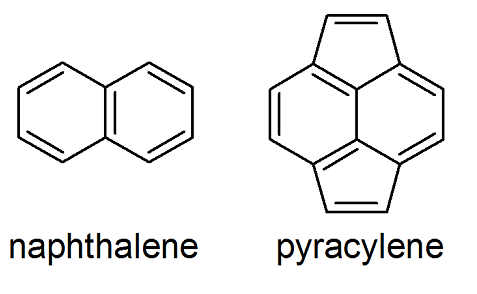
\includegraphics[width=90mm]{polycyclic.png}
\caption{Napthalene has two benzene rings with 2 carbon atoms is common. Even in complex polycylic hydrocarbons such as pyracylene, every ring shares only 2 carbon atoms.}
\label{fig:polycyclic}
\end{figure}

\subsubsection{Huckel's Rule}

The fourth condition is the most difficult. Due to the filling of quantum-mechanical electron orbitals, only aromatic molecules with 4n+2 electrons exhibit aromaticity. Compounds with 4n electrons exhibit anti-aromaticity. Groups of cycles add their delocalized electrons together to be one single $\pi$ conjugated system (see Figure ~\ref{fig:azulene}). This condition alone implies we must limit all ring systems to size of length 2, 6, or 10. However, Huckel's rule is mainly meant for monocyclic systems and has been shown to be inaccurate for many compounds containing more than three fused aromatic rings (see Figure ~\ref{fig:pyrene}) \cite{HuckelBad}. To account for this, in polycyclic systems, certain extensions to the rule have been added to better predict aromaticity \cite{HuckelExtension}.

\begin{figure}[ht!]
\centering
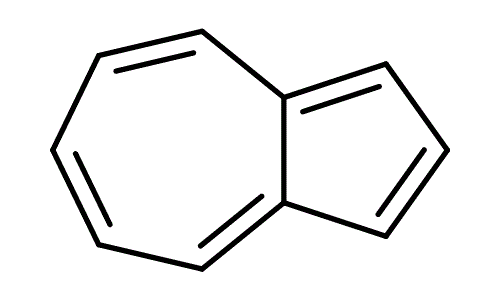
\includegraphics[width=50mm]{azulene.png}
\caption{Azulene, a structure composed of an aromatic heptene and pentene ring attached together. The total amount of $\pi$ contributing electrons is 10, 7 from heptene and 3 from pentene. Since 10 = 4n + 2 (where n = 2), Huckel's rule correctly predicts this structure to be aromatic.}
\label{fig:azulene}
\end{figure}

\begin{figure}[ht!]
\centering
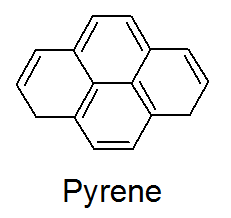
\includegraphics[width=50mm]{pyrene.png}
\caption{Although Pyrene has 16 conjugated electrons (which does not satisfy 4n + 2), it is still an aromatic molecule.}
\label{fig:pyrene}
\end{figure}



We choose to ignore Huckel's rule and any extensions. This is because even anti-aromatic compounds such as pentalene (8 contributing electrons) can be stabilized by adding the appropriate substituent. Either electron-donating or electron-withdrawing groups can be attached to the ring to allow aromaticity (see Figure ~\ref{fig:pentalene}). Additionally, it is possible to insert hereroatoms into the structure, such as nitrogen and sulphur. In addition to possibly making the molecules easier to synthesize, the nitrogen may add electrons to the conjugated system while leaving the switching behavior undisturbed \cite{v06} (see Figure, not existant yet%~\ref{fig:pyrrole}%). Although such substituents cannot, in every case, allow a stable molecule, they can in most cases. 

\begin{figure}[ht!]
\centering
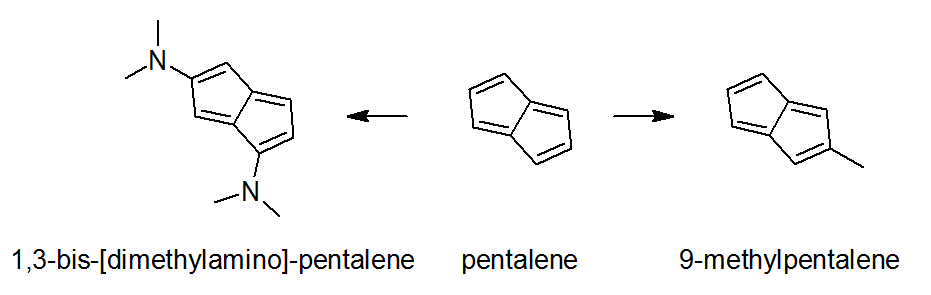
\includegraphics[width=160mm]{pentalene.png}
\caption{Pentalene can attach either the electron-donating Me \cite{methylPentalene} or N(Me)$_2$ \cite{nitrogenPentalene} group to achieve aromatic structure.}
\label{fig:pentalene}
\end{figure}

Despite ignoring Huckel's rule, we cannot discard this problem completely. Since ports do not need to contain a double bond, in some resonance structures of the same molecule, the amount of contributing electrons may be different (see Figure ~\ref{fig:badBenzene} and ~\ref{fig:badNapthalene}). Unless every resonance structure is aromatic, or at least every structure can be made aromatic by the same substituent, the molecule will not be able to realize all port assignments of the cell and is therefore unfit.  

\begin{figure}[ht!]
\centering
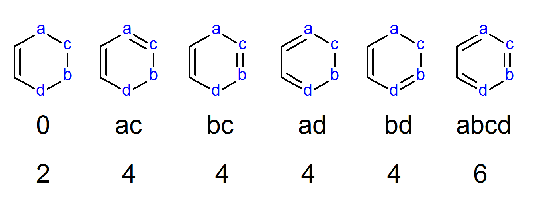
\includegraphics[width=130mm]{noSenseBenzene.png}
\caption{Below is a graph of benzene, which represents K5 of Hesselink's class 4 classification. The first line gives the structure, the second line the port assignment, and the third line the amount of electrons contributing to the ring. The problem here, is that only 2 and 6 are aromatic, and if we add substituents to stabilize the 4 electron structures, the 2 and 6 become unstable. }
\label{fig:badBenzene}
\end{figure}

\begin{figure}[ht!]
\centering
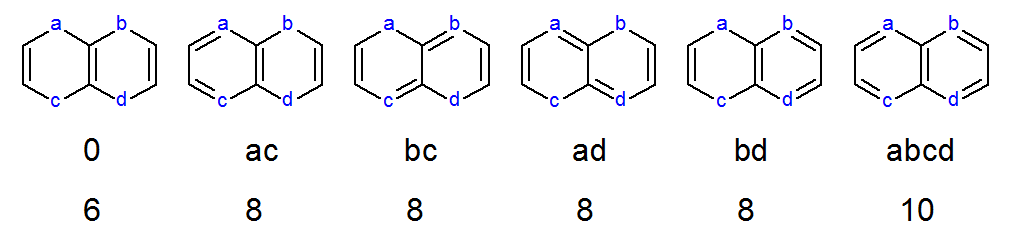
\includegraphics[width=150mm]{noSenseNapthalene.png}
\caption{Napthalene also can represent K5 of Hesselink's class 4 classification. This graph has the same problem as before. In fact, most graphs with 2 or more ports within a cycle system have this problem.}
\label{fig:badNapthalene}
\end{figure}

To account for this, we must ensure that each ring contains the same amount of electrons in every resonance structure. It is a difficult problem to determine which port placements could cause this. We have yet to discover a general solution. In any ring system, a single port is allowed. Since a double bond spans two atoms, every atom in the ring will still always contain a double bond, leaving the total number of bonds to remain constant. However, when two ports are added into a ring, or two rings are conjoined, it becomes unclear. For example, see Figure ~\ref{fig:checkMarks}. To ensure all results are manageable, all rings systems are restricted to one port. This means graphs such as napthalene, can only have a single port within the cycle. But if one graph contained two bridged napthalenes, each could contain a single port. This unnecessarily removes some graphs which could work, but it is a costly computation to determine for each graph whether it works. All other ports within the graph must be exo-cyclic. 

\begin{figure}[ht!]
\centering
\includegraphics[width=130mm]{checkMarks.png}
\caption{Benzene and Pentalene with two ports at various locations. Structures with a checkmark below indicate all resonance structures contain the same amount of double bonds. Structures with an x, indicate the opposite, and are unfit.}
\label{fig:checkMarks}
\end{figure}

Finally, graphs representing molecules must be connected. A disjoint graph more accurately represents two molecules rather than one. Although these restrictions do a good job of trimming out almost all unrealistic graphs, they are not absolute. Additionally, our restrictions make no attempt to ensure all graphs can be synthesized (more on this in Section 4). 

\section{Genetic Algorithm}

A genetic algorithm is used to search for graphs which apply to a given cell. The algorithm begins by randomly generating a population of graphs. Each starting graph has anywhere from rank to 31 nodes, and rank - 1 to 20 edges. There must be at least rank - 1 edges in order to connect the the minimum amount of nodes together. Graphs with fitness 0 or lower (normally arises from disconnected ports) are deleted and a new graph will take its place. This makes up the first generation.

In each iteration, the survivors of last generation's population must be chosen. This is done by selecting the best performing graphs (fitness-wise), along with a smaller amount of random graphs. Random graphs are added to ensure genetic diversity in the population. This sub-population now undergoes genetic operations such as mutation and crossover. 

The genetic algorithm has two terminating conditions. Either the maximum number of iterations has been reached, or some threshold of graphs which satisfy the cell has been reached. In some smaller cases, the genetic algorithm terminates immediately after generating the initial population, as it contained at least x graphs which satisfy the cell ( where x is the threshold of graphs desired).

Resulting graphs are converted to SMILES (cite here) (small molecular input line entry system) in order to be visualized. Conversion first involves finding a spanning tree of the graph. All edges in the original graph which are not in the spanning tree must be edges which complete a cycle. Therefore each node on either side of the edge is labeled as a cycle point. We then preform depth first search over the spanning tree, and append each nodes label as we reach it.

The ports are labeled by atoms with a P (normally reserved for a phosphorous atom). We need not label each port individually since Kekul\'e cells are invariant across port renaming \cite{H13}. The open source Chemistry Development Kit (citation) is used to parse the SMILES and generate a two-dimensional structure. Other than the ports, the structure resembles the hydrogen-suppressed carbon skeleton of the molecule.  

\subsection{Mutation}

Mutation involves randomly perturbing graphs to obtain new ones. We normally  generate enough mutants so that it is likely each graph will be mutated more than once. Mutations include:
\begin{enumerate}
\item Addition of a node
\item Removal of a random node, and all edges to it
\item Addition of a random edge \footnote{ Edges are randomly chosen until an edge is found that can be added without breaking our restrictions on the degree of vertices.}
\item Removal of a random edge
\item Port Extension
\end{enumerate}

Port extension involves adding a new node in the position of every port, and then adding the port connected to that node. This will always be viable since any port can have at most degree 2, and after port extension, the new nodes will have at most degree 3. This is often useful for spreading the ports out and allowing new edges without breaking our degree restrictions. Since each port will always have a degree of 1 after extension, each port can facilitate a new bond. See Figure ~\ref{fig:portExtension}.

\begin{figure}[ht!]
\centering
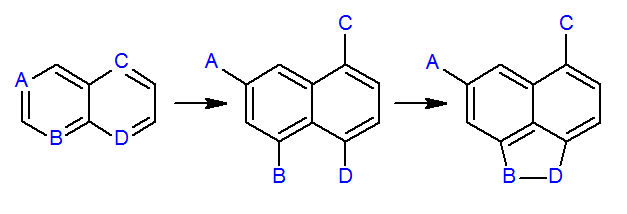
\includegraphics[width=110mm]{portExtension.png}
\caption{Napthalene (left) undergoing a port extension (center). Notice that after the port extension, it is now feasible to add an edge between B and D, which can then create Acenaphthene (right).}
\label{fig:portExtension}
\end{figure}

\subsection{Crossover}

Crossover begins by randomly selecting 2 graphs from the sub-population. These graphs are combined to create a new child graph. On average, each graph produces two children. Children receive all edges with both parents share, and have a 50\% chance to get any other edge found in one of the parents. This creates children which are a hybrid of both their parents.

\subsection{Fitness Function}

Fitness values are integers given to a graph. Any graphs cell can be calculated using Hesselink's procedure here: (explain a lot ). The fitness is calculated by iterating over the graphs cell compared to the cell we are evolving towards. For every port assignment they share, the fitness is incremented by one. For every port assignment that is missing, or is extra, fitness is decremented one point. If a cell is empty, with no port assignments \footnote{This can happen when the genetic algorithm creates a graph which has a (non-port) vertex with no edges to it (degree 0). There is no way for this graph to have a Kekul\'e structure since the lone vertex can never have a double bond.}, it is discarded.

\subsection{Cycle Detection}

Cycles are detected using an upper bounded implementation of the 'flooding' algorithm (need cite here). In the flooding algorithm, each node sends out a packet to all if it's neighbors. Any time a node receives a packet, it appends its name and sends the new packet to all of its neighbors. Packets are not sent back to the node who it was just received it from. If at any time a packet has been appended by the same node twice, we have found a cycle. As soon as a packet finds a cycle, the packet is discontinued. Packets of length $>$ 12 are also discontinued. This introduces the error that a graph could contain a cycle of length 13. The amount of computation time saved is usually worth it, considering how unlikely a cycle of length 13 or greater is. 

Some optimizations can be made considering the subset of all possible graphs we are dealing with. Packets only begin on nodes with degree of 3, as this is guaranteed to find all cycles. Every point within a cycle has a degree of 2, so if that cycle is connected to any other node, then at least one of that cycles nodes will have a degree of 3. If there are no nodes with degree of 3, the graph either contains no cycles, or the graph is one big cycle. Therefore, in this case, we only start a single packet at one random node. This is still slow.

\subsection{Cycle Extension and Contraction}
Cycle extension is done by inserting two additional carbon atoms into the cycle at the same position (see Figure ~\ref{fig:cycleExtension}). This has no effect on the Kekul\'e cell as the two atoms are conjugated with the rest of the ring and simply expand it. This procedure is nearly identical to operation v of \cite{v06}. Care must be taken to not select two nodes which also are a part of another cycle, as the resulting graph will contain unrealistic bonding distances and cycle connectivity. The opposite procedure can be used to contract cycles. Contraction is only possible if there are two neighboring nodes with no edges outside the ring. Graphs with un-alterable cycles outside our limits are excluded.

\begin{figure}[ht!]
\centering
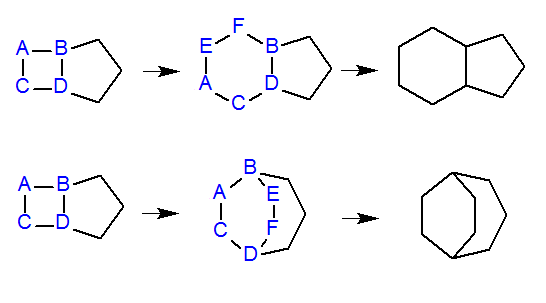
\includegraphics[width=90mm]{cycleExtension.png}
\caption{This shows the extension of the left 4 cycle into a proper 6 cycle. The top half shows a correct procedure, selecting to add nodes between A and B. The bottom half shows the incorrect procedure of adding two nodes in between B and D. Double bonds are excluded from this diagram for clarity.}
\label{fig:cycleExtension}
\end{figure}

\subsection{Connecting a Disjoint Graph}
A disjoint graph is not an accurate representation of a molecule. Luckily, disjoint graphs can often be connected using the following procedure. If we add internal vertices which must always conjugate ’within’ themselves, they will not interfere with the cell. For example, see Figure ~\ref{fig:disjoint}.

\begin{figure}[ht!]
\centering
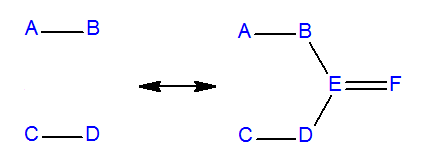
\includegraphics[width=90mm]{disjoint2.png}
\caption{Process used to turn a disjoint graph to a connected graph with the same cell. Two new nodes E and F can be added which always conjugate to each other.}
\label{fig:disjoint}
\end{figure}

In the right-hand graph of Figure ~\ref{fig:disjoint}, F is not a port and so must always contain a double bond. The only other node which is available to form a double bond with F is E, so in every resonance structure of this molecule E and F will contain a double bond with each other (as shown in right diagram). Therefore d or b can never form a double bond with their new edge (that would result in two adjacent double bonds), and the Kekul\'e cell has not been changed. This now resembles a stable connected molecule. This procedure is similar to Operation iii and vi of [3].

\subsection{Minor Implementation Details} 

\subsubsection{The Bit Vector}

A Bit Vector (or Bit array, bitmap, bitset, bitstring, etc) is an array data structure that compactly stores bits. It can be used to implement a simple set data structure. Although the Bit Vector is an array, the entire set can be contained with a single binary integer. Every 1 indicates the presence of something, and 0, the absence. For example, 0001 0101 (or 21) is a set of three elements. Node 1, node 3, and node 5. 

Because the entire array is within an integer, it is very easy and computationally quick to perform certain operations. You can add or remove a node from your set by simple addition / subtraction. You can iterate through the set by starting at 1 and performing left bit shifts. You can use bitwise AND to take the intersection of two sets, or to check whether a set contains a given element (Figure 1). You can add two sets together with bitwise OR. You can even take the symmetric difference between two sets with XOR.

Whenever you can distinguish elements of your set with a single number, and your sets are not large enough to overflow an integer, you should consider using bit vectors. They are extremely compact, versatile, and quick.

In this application, bit vectors represent sets of nodes, as in the example above. They are also used to represent edges (a set of nodes with 2 elements) of graphs. 

\subsubsection{The Cell}

A port assignment is the set of ports which have a double bond in a particular Kekul\'e structure. In this application, cells have two purposes. 

\begin{enumerate}
\item A cell can hold an array of port assignments, one for every possible resonance structure of that molecule. It can be used to fully describe the electrical switching behavior of a molecule.
\item A cell can hold an array of edges. Each edge is represented using a Bit Vector. In this way, a cell con constitute an entire graph.
\end{enumerate}


\subsection{Additional Note}

It should be noted that rather than using the genetic algorithm to approximate a solution (as seen in most applications), an answer generated by it is only useful if it found an actual solution. However, for all cells of rank \textless 6 and most cells of rank 6, the genetic algorithm can converge to multiple solutions for a given cell. 

\section{Results}

Most graphs produced by the algorithm can be feasibly realized in stable molecules. However, results are not perfect. As stated previously, rings of sizes other than 6 are not always stable. 

Planarity? The second condition is another current drawback. Since the cycle detection algorithm needs an upper bound, in rare cases, cycles above this limit can appear. This can cause other smaller cycles which share more than two atoms with the large cycle to not be detected. Additionally, some bonding distances may be unrealistic. For examples of both, see Figure ~\ref{fig:unrealistic}.

\begin{figure}[ht!]
\centering
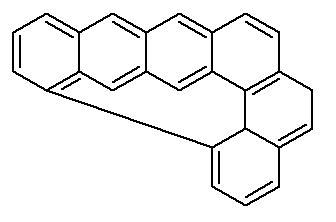
\includegraphics[width=70mm]{unrealistic.png}
\caption{An example of an unrealistic molecule that could be generated by the genetic algorithm. There is a long stretched bond from the first benzene (top left) to the last benzene (bottom right). This stretched bond completes a cycle that has a length of 9. If the cycle detection algorithm had a limit of 8, this graph could be a result. Not only is the stretched bond unrealistic, but the cycle it creates shares up to 3 atoms with some rings.}
\label{fig:unrealistic}
\end{figure}
 
In most small cases (ports \textless 6), the genetic algorithm is able to obtain atleast 10 different graphs which satisfy the cell immediately. For some of the later classifications of rank 5, and cells of rank 6 or higher, it can take longer. Some cells of rank 6 it is unable to find a graph for. As it is possible that no such realistic graph exists for some cells, it is difficult to determine whether a solution exists. The number of nodes is currently maxed at 31 nodes, as nodes are stored in a bit array, which would overflow the integer at 32.

Below is graphs for all cells of rank 4 and 5. Double bonds are excluded from the graphs shown below, as only one resonance structure could be seen at a time. Some graphs may have cells different than the title below them. This is because their cells can be port translated to achieve the classified cell. This is acceptable since switching behaviour is invariant across port translation \cite{HH13}. As stated previously, the genetic algorithm is capable of coming to multiple solutions for each cell, and the ones shown below are simply ones selected by us. Notice the trend that as the Kekul\'e cell number increases, the Kekul\'e cell becomes longer. This means more resonance structures of each graph, and more connections between atoms. The higher amount of connectivity required in each cell makes it so the next graph is usually more difficult to find than the last one. Looking at Figures ~\ref{fig:rank5Results1} and ~\ref{fig:rank5Results2}, it is easy to see that the graphs get bigger and more complex as the cell number increases. 

\begin{figure}[ht!]
\centering
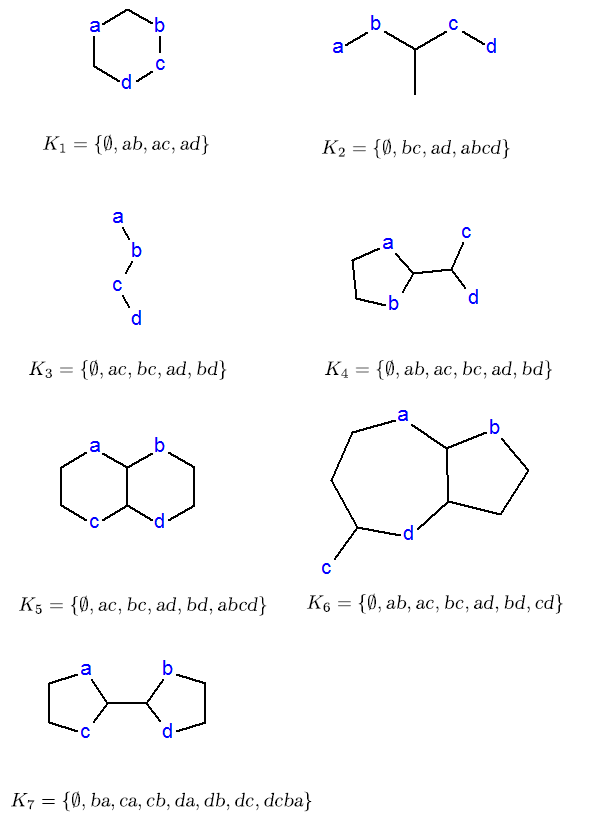
\includegraphics[width=130mm]{rank4Results.png}
\caption{Realistic Graphs for each cell in Hesselink's classification of all cells with rank 4. K$_1$ resembles benzene, K$_5$ napthalene, and K$_6$ azulene.}
\label{fig:rank4Results}
\end{figure}

\begin{figure}[ht!]
\centering
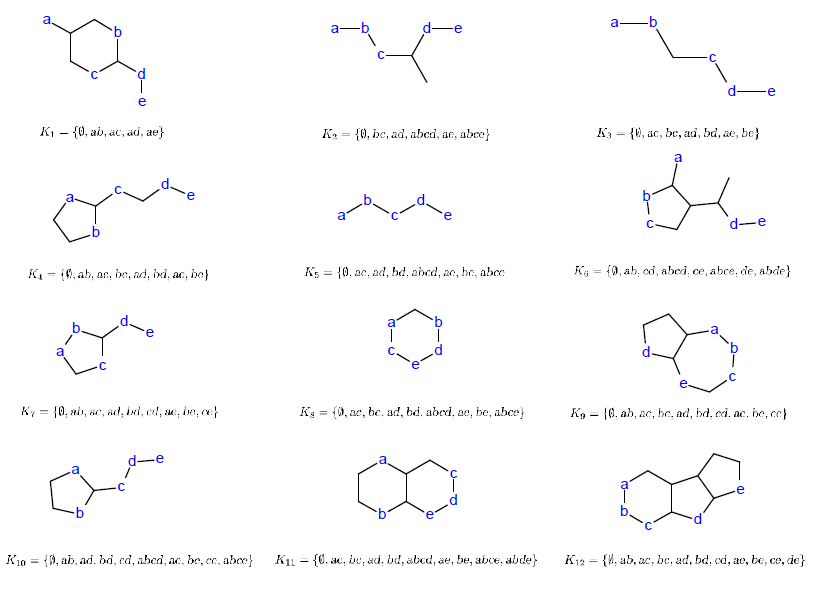
\includegraphics[width=160mm]{rank5Results1.png}
\caption{Realistic Graphs for the first 12 cells in Hesselink's classification of all cells with rank 5. K$_1$ and K$_8$ resembles benzene, K$_{11}$ napthalene, and K$_9$ azulene.}
\label{fig:rank5Results1}
\end{figure}

\begin{figure}[ht!]
\centering
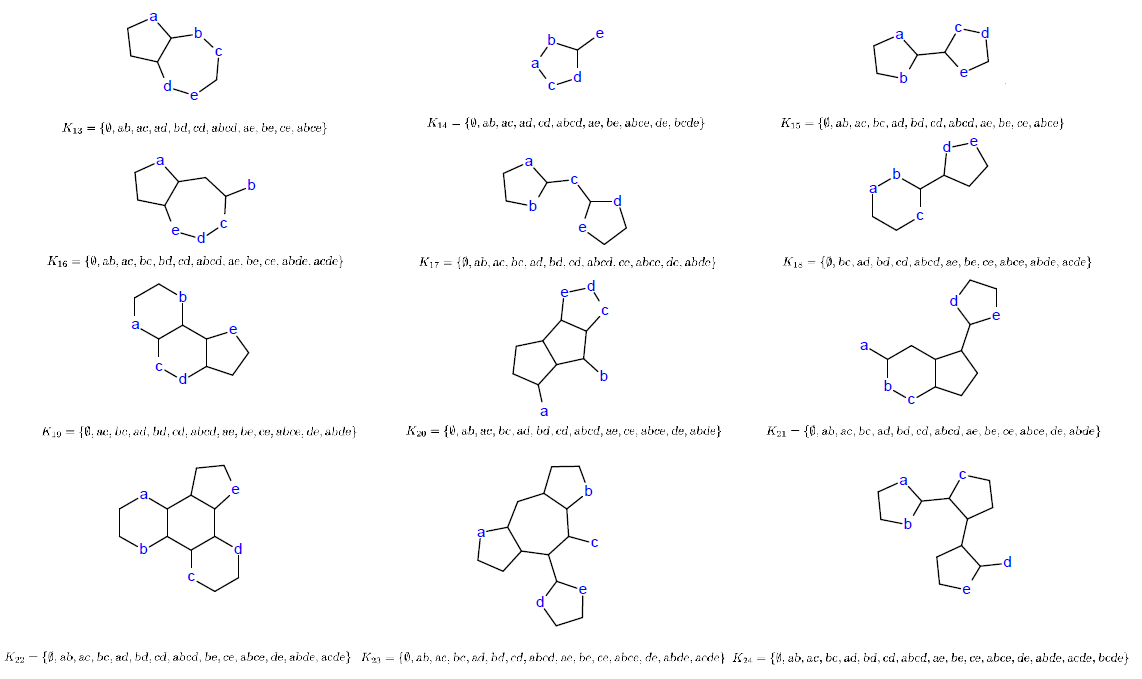
\includegraphics[width=160mm]{rank5Results2.png}
\caption{Realistic Graphs for the second half of cells in Hesselink's classification of all cells with rank 5. K$_{13}$, K$_{16}$ azulene both resemble azulene.}
\label{fig:rank5Results2}
\end{figure}

Finding graphs for cells of higher ranks builds on this challenge. Not only is every graph larger, but there must be an additional atom with degree of 2. The number of combinations increases drastically, with 3 classes of rank 3, 7 classes of rank 4, 24 classes of rank 5, and 214 classes of rank 6. When attempting to find graphs for all cells of rank 6, we were able to find graphs for X out of 214. All graphs found can be viewed here: (website).

Increasing the number of nodes to above 32 will likely yield more results in some cases, however, it will lower performance. It is possible many graphs do not have a realistic graph which matches it's cell.

Even if all graphs produced represent stable molecules, there are additional problems. Each hydrocarbon must be able to be easily synthesized for it to be of any use. Analysis on the synthesis of hydrocarbons here.

Polycylic aromatic hydrocarbons are commonly produced as byproducts of fuel burning, and have been classified as carcinogenic, mutagenic, and teratogenic. This could pose a challenging problem if we wish to use large aromatic hydrocarbons in circuitry. 

There are many possible improvements in this area. The number of nodes could be increased to allow larger graphs. Although this would increase the amount of computation required, perhaps it is possible to implement a more efficient cycle detection algorithm, or even calculate fitness on every 2nd iteration of the genetic algorithm. These changes may allow even more results to be yielded from a heuristic genetic algorithm based approach.

%\section{Conclusion}

\begin{thebibliography}{abrv}

\bibitem{H13} W. H. Hesselink, Graph Theory for alternating hydrocarbons with attached ports. Indagationes Mathematicae, Elsevier, 24:115141, 2013.
\bibitem{HH13} W.H. Hesselink, J.C. Hummelen, H.T. Jonkman, H.G. Reker, G.R. Renardel de Lavalette, M.H. van der Veen, Kekule Cells for Molecular Computation. Cornell University Library Online, 2013.
\bibitem{v06} M.H. van der Veen. $\pi$-Logic. PhD thesis, University of Groningen, May 2006.
\bibitem{HK88} A.J. Heeger, S. Kivelson, J.R. Schrieffer, and W.-P Su. Solitons in conducting polymers, Rev. Mod. Phys.,60:781, 1988.
\bibitem{Moore} G. E. Moore, Cramming more components onto integrated circuits. Electronics Magazine. p. 4. Retrieved 2006-11-11. 
\bibitem{MooreEnd} C. A. Mack, Fifty Years of Moore's Law. IEEE Transactions on semiconductor manufacturing, 24:2 2011.
\bibitem{OmniConj} M. H. van der Veen, M. T. Rispens, H. T. Jonkman, and J. C. Hummelen, Molecules with Linear $\pi$-Conjugated Pathways between all Substituents: Omniconjugation. Adv. Function Mater, 14:3, 2004.
\bibitem{openPath} S.N. Yalirahi, M.A. Ratner, Interplay of topology and chemical stability on the electronic transport of molecular junctions, Ann. New York Acad. Sci. 960 (2002) 153.
\bibitem{9} J. Reichert, R. Ochs, D. Beckmann, H. B. Weber, M. Mayor, H. von Löhneysen,Phys. Rev. Lett. 2002, 88, 176804. 
\bibitem{10} A. Aviram, M. A. Ratner, Chem. Phys. Lett. 1974, 29, 277.
\bibitem{11} D. B. Strukov, K. K. Likharev, Nanotechnology 2005, 16, 137.
\bibitem{12} Y. Karzazi, J. Cornil, J. L. Brédas, J. Am. Chem. Soc. 2001, 123, 10076.
\bibitem{13} J. M. Tour, M. Kozaki, J. M. Seminario, J. Am. Chem. Soc. 1998, 120, 8486.
\bibitem{14} A. Aviram, J. Am. Chem. Soc. 1988, 110, 5687.
\bibitem{15} H. W. Ch. Postma, T. Teepen, Z. Yao, M. Grifoni, C. Dekker, Science 2001, 293, 76.
\bibitem{16} C. Joachim, J. K. Gimzewski, Chem. Phys. Lett. 1997, 265, 353.
\bibitem{17} T. D. Anthopoulos, C. Tanase, S. Setayesh, E. J. Meijer, J. C. Hummelen, P. W. M. Blom, D. M. de Leeuw, Adv. Funct. Mater. 2004, 16, 2174.
\bibitem{18} G. M. Tsivgoulis, J.-M. Lehn, Chem. Eur. J. 1996, 2, 1399.
\bibitem{19} J. J. D. de Jong, L. N. Lucas, R. M. Kellogg, J. H. van Esch, B. L. Feringa, Science 2004, 304, 278.
\bibitem{20} A. P. de Silva, H. Q. N. Gunaratne, C. P. McCoy, Nature 1993, 364, 42.
\bibitem{21} F. M. Raymo, S. Giordani, J. Org. Chem. 2003, 68, 4158.
\bibitem{22} K. Rurack, A. Koval'chuck, J. L. Bricks, J. L. Slominskii, J. Am. Chem. Soc. 2001, 123, 6205.
\bibitem{23} D. Parker, J. A. G. Williams, Chem. Commun. 1998, 245.
\bibitem{24} A. P. de Silva, I. M. Dixon, H. Q. N. Gunaratne, T. Gunnlaugsson, P. R. S. Maxwell, T. E. Rice, J. Am. Chem. Soc. 1999, 121, 1393.

\bibitem{HuckelBad} Roberts, J. D., Streitwieser Jr, A., and Regan, C. M. Small-Ring Compounds. X. Molecular Orbital Calculations of Properties of Some Small-Ring Hydrocarbons and Free Radicals. Journal of the American Chemical Society, 74(18), 4579-4582. 1952.

\bibitem{HuckelExtension} Kruszewski, J., and Krygowski, T. M. An Extension of the Hückel 4N+ 2 Rule to Polycyclic Non-alternant Conjugated Hydrocarbons. Canadian Journal of Chemistry, 53(6), 945-951. 1975.

\bibitem{methylPentalene} Hafner, K., Donges, R., Goedecke, E. and 
Kaiser, R. Concerning Pentalene, 2-Methylpentalane, and 1,3-
Dimethylpentalene. Angew. Chem. Int. Ed. Engl., 12: 337-339. 1973.

\bibitem{nitrogenPentalene} Hafner, K., Bangert, K. F. and Orfanos, V 1,3-Bis(dimethylamino)pentalene. Angew. Chem. Int. Ed. Engl., 6: 451–452. 1967.

\end{thebibliography}

\end{document}
